\documentclass[tikz,border=5pt]{standalone}
\usepackage[T1]{fontenc}
\usepackage{lmodern,amsmath,amssymb}
\usetikzlibrary{arrows.meta,calc,positioning,fit,backgrounds,shapes.geometric,matrix,decorations.pathreplacing,patterns}
\definecolor{ink}{gray}{0.08}
\definecolor{wash}{gray}{0.965}
\definecolor{soft}{gray}{0.45}
\tikzset{box/.style={draw=ink,line width=.65pt,fill=white,align=center,inner sep=4pt,outer sep=0pt,font=\small},flow/.style={draw=ink,line width=.65pt,-{Latex[length=1.8mm,width=1.3mm]},rounded corners=2pt},annotation/.style={font=\scriptsize,text=soft,align=center},groupbox/.style={draw=soft,dashed,line width=.45pt,fill=wash}}
\begin{document}
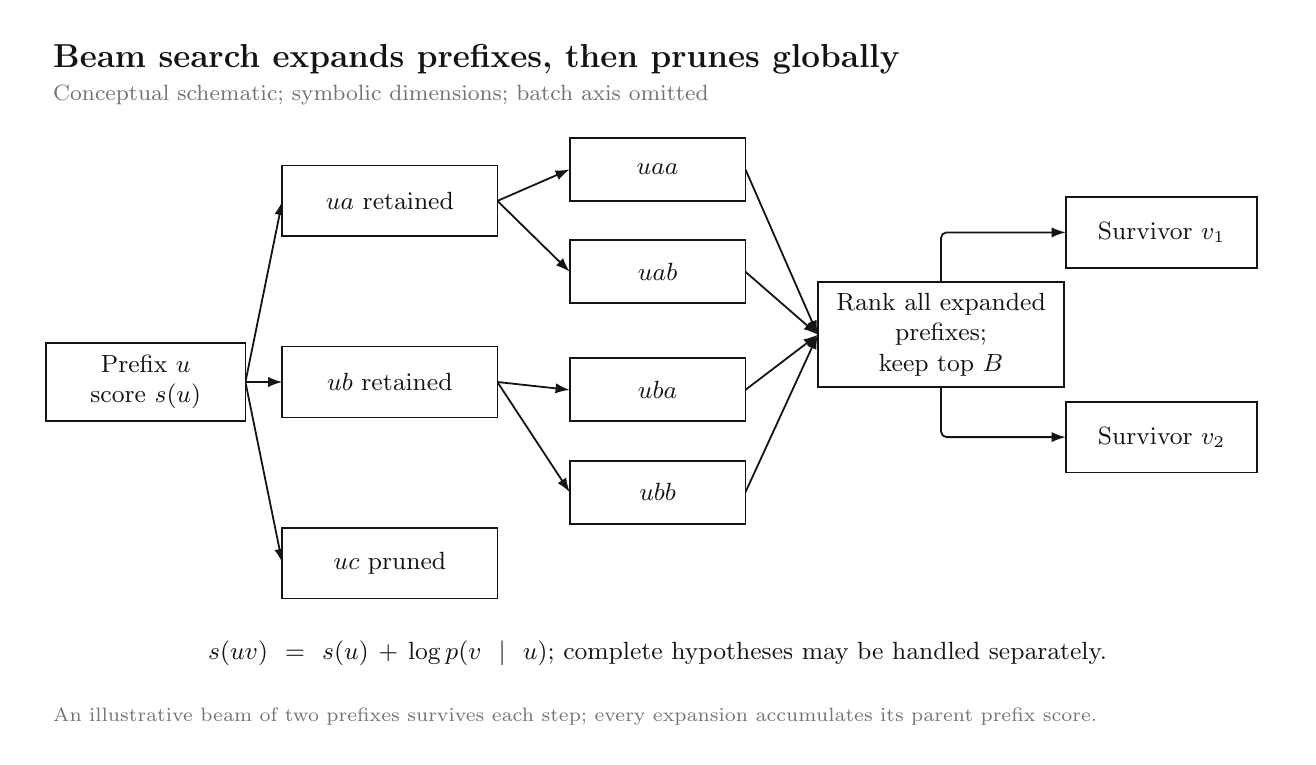
\begin{tikzpicture}[x=1cm,y=-1cm,font=\rmfamily,text=ink]

\path[use as bounding box] (0,0) rectangle (16,9);
\node[anchor=west,font=\large\bfseries] at (.2,.4) {Beam search expands prefixes, then prunes globally};
\node[anchor=west,font=\footnotesize,text=soft] at (.2,.85) {Conceptual schematic; symbolic dimensions; batch axis omitted};
\begin{pgfonlayer}{background}
\end{pgfonlayer}
\node[box,minimum width=2.5cm,minimum height=1.0cm,text width=2.25cm] (seed) at (1.5,4.5) {Prefix $u$\\score $s(u)$};
\node[box,minimum width=2.7cm,minimum height=0.9cm,text width=2.45cm] (a) at (4.6,2.2) {$ua$ retained};
\node[box,minimum width=2.7cm,minimum height=0.9cm,text width=2.45cm] (b) at (4.6,4.5) {$ub$ retained};
\node[box,minimum width=2.7cm,minimum height=0.9cm,text width=2.45cm] (c) at (4.6,6.8) {$uc$ pruned};
\node[box,minimum width=2.2cm,minimum height=0.8cm,text width=1.9500000000000002cm] (aa) at (8.0,1.8) {$uaa$};
\node[box,minimum width=2.2cm,minimum height=0.8cm,text width=1.9500000000000002cm] (ab) at (8.0,3.1) {$uab$};
\node[box,minimum width=2.2cm,minimum height=0.8cm,text width=1.9500000000000002cm] (ba) at (8.0,4.6) {$uba$};
\node[box,minimum width=2.2cm,minimum height=0.8cm,text width=1.9500000000000002cm] (bb) at (8.0,5.9) {$ubb$};
\node[box,minimum width=3.1cm,minimum height=1.2cm,text width=2.85cm] (rank) at (11.6,3.9) {Rank all expanded\\prefixes; keep top $B$};
\node[box,minimum width=2.4cm,minimum height=0.9cm,text width=2.15cm] (s1) at (14.4,2.6) {Survivor $v_1$};
\node[box,minimum width=2.4cm,minimum height=0.9cm,text width=2.15cm] (s2) at (14.4,5.2) {Survivor $v_2$};
\node[align=center,inner sep=0pt,outer sep=0pt,font=\small,minimum width=13.5cm,minimum height=0.6cm,text width=13.25cm] (note11) at (8,7.95) {$s(uv)=s(u)+\log p(v\mid u)$; complete hypotheses may be handled separately.};
\begin{pgfonlayer}{background}
\draw[flow] (seed.east) -- (a.west);
\draw[flow] (seed.east) -- (b.west);
\draw[flow] (seed.east) -- (c.west);
\draw[flow] (a.east) -- (aa.west);
\draw[flow] (a.east) -- (ab.west);
\draw[flow] (b.east) -- (ba.west);
\draw[flow] (b.east) -- (bb.west);
\draw[flow] (aa.east) -- (rank.west);
\draw[flow] (ab.east) -- (rank.west);
\draw[flow] (ba.east) -- (rank.west);
\draw[flow] (bb.east) -- (rank.west);
\draw[flow] (rank.north) -- (11.6,2.6) -- (s1.west);
\draw[flow] (rank.south) -- (11.6,5.2) -- (s2.west);
\end{pgfonlayer}
\node[anchor=west,align=left,font=\scriptsize,text=soft,text width=15.6cm] at (.2,8.75) {An illustrative beam of two prefixes survives each step; every expansion accumulates its parent prefix score.};
\end{tikzpicture}
\end{document}
